\section{Hybrid approach}
\label{sec:hybrid}
Phase~1 left two strong but different predictors of the 2\,s drift
magnitude: Lasso on 104 hand-made features (mean test MAE 2.50\,cm,
$R^2=0.76$) and the physics feature $\mathrm{phys\_mag}$, the drift that a
training-flight bias calibration predicts (mean $R^2=0.82$). R2's IMU
networks alone do not reach either (E2 LSTM: 3.52\,cm, $R^2=0.51$). The
hybrid question is therefore whether learned and hand-made knowledge add up,
and in particular whether a network can correct what physics misses.

\subsection{Architecture}
All hybrids use intermediate fusion~\cite{r4baltrusaitis2019}. Each active
branch maps its input to a 64-number embedding, following the shared
contract: R2's LSTM on the raw $(6,400)$ window, a two-layer MLP on the 104
normalised features plus the four standardised physics numbers, and R3's
camera CNN on the $(3,64,64)$ frames. The embeddings are concatenated, mixed
by one Linear--ReLU--Dropout layer to 64 numbers, and mapped by R2's shared
regression head to $z$. Three presets are built from one class with branch
flags (Fig.~\ref{fig:hybrid-arch}):
\begin{itemize}
\item \textbf{H1} (E3): IMU + features + physics, $\hat y=\bar y+s\,z$.
\item \textbf{H2} (E4, main): physics prior plus learned residual,
  \begin{equation}
  \hat y = a\,\mathrm{phys\_mag} + b + s\,z ,
  \end{equation}
  where $a,b$ are least squares on the inner-training windows and the head's
  last layer is initialised to zero, so the untrained model \emph{is} the
  physics prediction~\cite{r4zeng2020,r4johannink2019}.
\item \textbf{H3} (E6): IMU + camera, $\hat y=\bar y+s\,z$. A missing camera
  input gives a zero embedding.
\end{itemize}
$\bar y$ and $s$ are the training mean and standard deviation of the target
(of the residual for H2). The network therefore predicts standardised
values and never has to learn the 1.2\,m offset of $\mathrm{err\_mag\_m}$.
The loss is MSE in these standardised units. Training reuses R2's policy:
AdamW (lr $10^{-3}$, weight decay $10^{-4}$), dropout 0.3, ReduceLROnPlateau,
gradient clipping at 1, early stopping (patience 15) on R1's validation
block, and best-checkpoint restore. For H2 only, the epoch-0 (physics)
checkpoint is a valid choice. E7 adds R3's ten optical-flow numbers to the
feature branch of whichever of E3/E4/E6 had the lowest \emph{validation}
MAE; this was E4. E4vec repeats E4 with the four-value head (magnitude
and $d_x,d_y,d_z$) for R5's drift correction. E4cnn repeats E4 with R2's
1D-CNN as the IMU encoder. For the branch ablation, IMUlstm and IMUcnn
switch the feature branch off, so only raw IMU is used, with the same
target scaling. Every experiment ran on both folds with seeds 42, 43 and 44.

\begin{figure}[t]
\centering
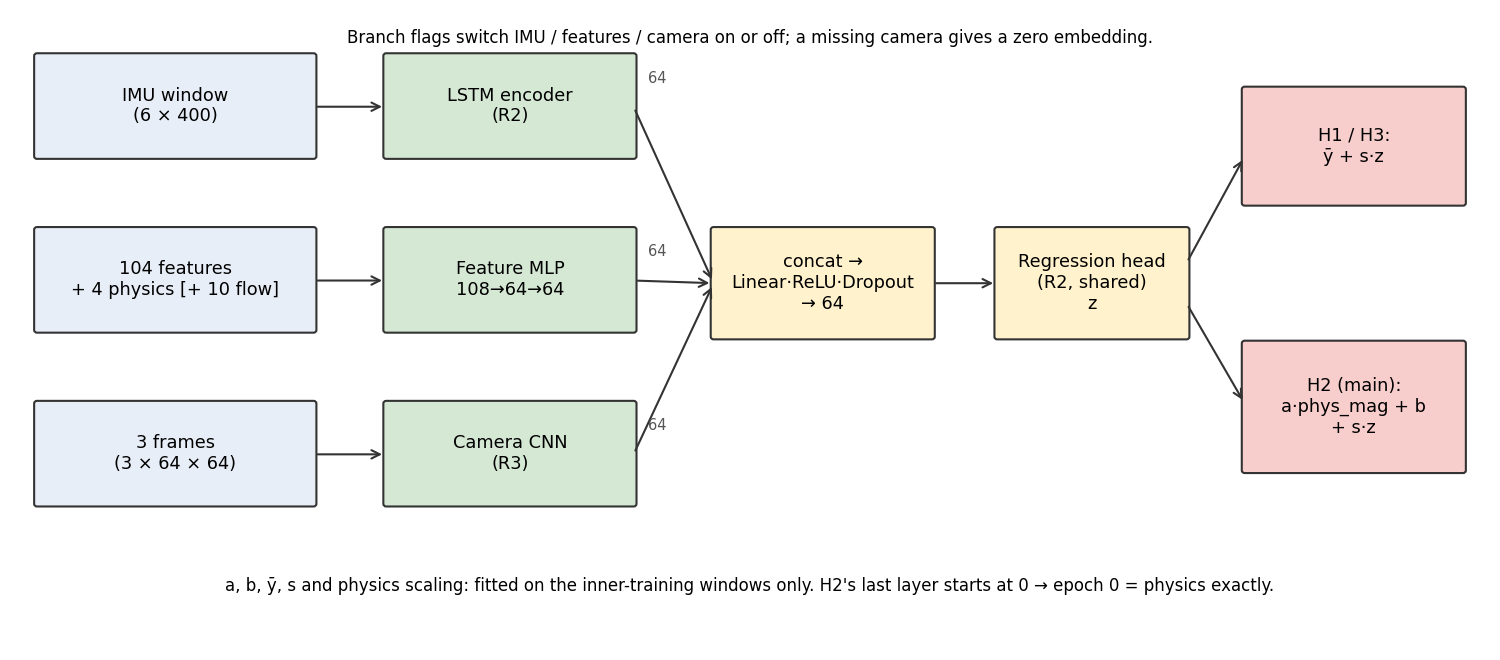
\includegraphics[width=\columnwidth]{../../figures/dl/hybrid_architecture.png}
\caption{Hybrid fusion. Branch flags switch IMU, features and camera on or
off; H2 adds the network output to the fitted physics prediction.}
\label{fig:hybrid-arch}
\end{figure}

\subsection{Results}
Table~\ref{tab:hybrid} reports test-flight scores with the seed spread.
The physics-only row uses the same $a,b$ as H2.

\begin{table}[t]
\centering
\caption{Test MAE (cm) and mean $R^2$; networks: mean $\pm$ std over 3
seeds. ``wu'': 10-epoch warm-up (sensitivity run, see text).}
\label{tab:hybrid}
\begin{tabular}{lccc}
\hline
Model & leave MH\_01 & leave MH\_02 & Mean $R^2$ \\
\hline
Mean baseline & 4.40 & 4.65 & $-0.03$ \\
Lasso (Phase 1) & 2.59 & 2.42 & 0.76 \\
Physics only & 2.25 & \textbf{1.97} & \textbf{0.82} \\
\hline
\multicolumn{4}{l}{\emph{Branch ablation: raw IMU only}} \\
IMUlstm & $2.99\pm0.14$ & $4.38\pm0.06$ & 0.31 \\
IMUcnn & $2.61\pm0.12$ & $2.58\pm0.12$ & 0.72 \\
\hline
\multicolumn{4}{l}{\emph{Hybrids}} \\
E3 H1 & $2.53\pm0.07$ & $3.77\pm0.10$ & 0.53 \\
E3 H1, wu & $2.59\pm0.05$ & $2.69\pm0.07$ & 0.73 \\
E4 H2, LSTM (main) & $2.24\pm0.02$ & $2.07\pm0.02$ & \textbf{0.82} \\
E4cnn H2, CNN & $\mathbf{2.23\pm0.02}$ & $2.03\pm0.05$ & \textbf{0.82} \\
E4vec H2, 4 outputs & $2.22\pm0.03$ & $2.09\pm0.03$ & 0.82 \\
E6 H3 & $2.98\pm0.33$ & $4.07\pm0.52$ & 0.38 \\
E6 H3, wu & $2.82\pm0.10$ & $2.88\pm0.03$ & 0.64 \\
E7 H2 + flow & $2.24\pm0.01$ & $2.11\pm0.12$ & 0.81 \\
\hline
\multicolumn{4}{l}{\emph{Lasso under the Phase 2 validation rule (diagnostic)}} \\
104 features & 2.56 & 4.63 & 0.32 \\
104 + 4 physics & 2.55 & 3.98 & 0.50 \\
\hline
\end{tabular}
\end{table}

\textbf{H2 is the best Phase 2 model, and it matches physics.} H2 beats
Phase~1 Lasso on both folds (mean $R^2$ 0.82 vs 0.76) with a seed spread
of only 0.01--0.05\,cm. It does not beat physics alone. With MH\_01 as
the test flight it is 0.01--0.02\,cm better, smaller than the seed
spread. With MH\_02 as the test flight it is 0.07--0.10\,cm worse. The
result holds for both encoders: LSTM 2.15\,cm and CNN 2.13\,cm mean MAE.
The physics backbone, not the encoder, decides the result. Splitting the
MH\_02 test flight into take-off (first 20\,\%) and the rest shows where
H2 (LSTM) loses: it is slightly better than physics after take-off
(1.86--1.92 vs 1.94\,cm) but worse during take-off (2.66--2.80 vs
2.05\,cm). Physics alone is at $R^2=0.82$, against the 0.83 ceiling
measured in Phase~1 for any bias-based predictor, so little learnable
signal remains.

\textbf{Why the network does not improve on physics: the validation
block.} R1 holds out the last 20\,\% of each training flight, mostly
landing. Its label standard deviation is 2.2--3.6\,cm, against
6.3--8.8\,cm on the training windows, and physics alone has
$R^2\approx0$ on it. Checkpoint selection therefore rests on a segment
with almost no learnable signal and no take-off motion
(Fig.~\ref{fig:hybrid-curves}). For H2 this is harmless: the zero-initialised
correction lets early stopping fall back to physics. Direct models have
no such fallback. On the MH\_02 test fold, H1 and IMUlstm kept their
epoch-1 checkpoint in all three seeds, an almost untrained network,
while their training error was still falling.

\textbf{Warm-up sensitivity.} After observing this, we re-ran the
direct hybrids with no checkpoint allowed before epoch 10, the point
where the \emph{training} curves flatten. Test data played no part in
choosing 10. H1 improves from $R^2$ 0.53 to 0.73, close to Phase~1
Lasso, and H3 improves from 0.38 to 0.64, with its seed spread falling
from 0.39 to 0.05\,cm. Validation MAE got \emph{worse} in these runs
while test MAE got better, which confirms that the landing block
mis-ranks checkpoints. Both versions are reported. The warm-up rows are a
sensitivity analysis, not a replacement.

\textbf{Encoders and branches.} With the target standardised, the raw-IMU
1D-CNN reaches $R^2$ 0.72 (2.60\,cm). That is close to Phase~1 Lasso on
104 hand-made features, and far from the failure of the unscaled E1. The
raw-IMU LSTM is weaker (0.31) and more exposed to the early-stopping
problem. Adding the 104 features and the physics numbers as \emph{inputs}
(H1, warm-up) gives about the same score as the CNN alone (0.73). Using
physics as the \emph{output backbone} (H2) adds the most, reaching 0.82
with either encoder. The camera adds variance, not accuracy (H3), and the
optical-flow numbers change H2 by less than the seed spread (E7).

\textbf{ML under the same rules.} Lasso refitted on the same
inner-training windows, with alpha chosen on the same validation block,
degrades badly. The landing block favours a large penalty. Without physics
on the MH\_02 test fold, Lasso zeroes every feature. With physics, it
keeps only $\mathrm{phys\_mag}$ and shrinks its weight. The physics
numbers still help (mean MAE 3.59 to 3.27\,cm). H2 is protected because
its physics part is unpenalised least squares. Phase~1's time-block
tuning brings Lasso with physics to about 2.15\,cm in a side check, level
with H2. The advantage shown here is robustness to the selection rule,
not extra signal.

\begin{figure}[t]
\centering
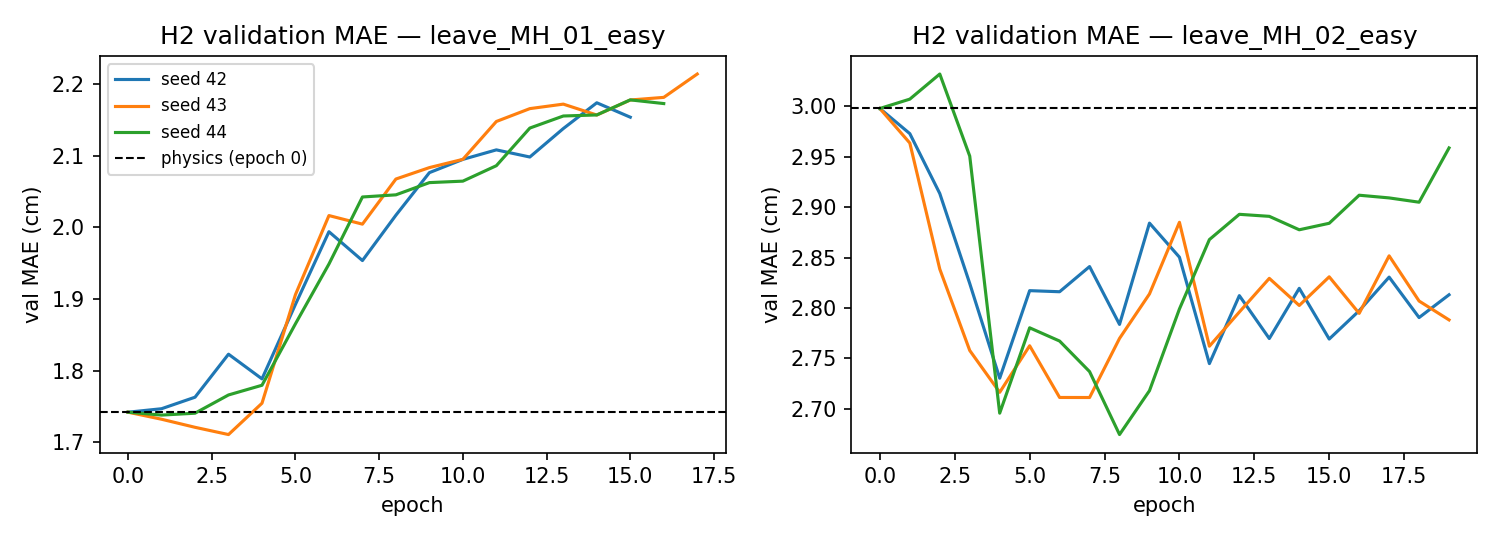
\includegraphics[width=\columnwidth]{../../figures/dl/hybrid_h2_curves.png}
\caption{H2 validation MAE per epoch; the dashed line is physics alone
(epoch 0).}
\label{fig:hybrid-curves}
\end{figure}

\subsection{Drift correction and caveats}
For drift correction, the physics vector alone reduces the mean end-point
error vector from 121 and 120\,cm to 6.6 and 5.5\,cm. E4vec gives 6.4
and 5.7\,cm (mean of 3 seeds), a tie within the seed spread. As in
Phase~1, labels and physics start each window from the ground-truth
state, so these numbers are an upper bound on what a deployed system
would see. Only two flights are available, so every comparison rests on
two folds.
